\documentclass[pdflatex,sn-mathphys-ay]{sn-jnl}
\usepackage{graphicx,amsmath,amssymb,amsthm,booktabs,multirow}
\usepackage[T1]{fontenc}
\usepackage{lmodern}
\input{glyphtounicode}
\pdfgentounicode=1
\theoremstyle{thmstyleone}
\newtheorem{theorem}{Theorem}
\newtheorem{lemma}[theorem]{Lemma}
\newtheorem{corollary}[theorem]{Corollary}
\newtheorem{proposition}[theorem]{Proposition}
\theoremstyle{thmstyletwo}
\newtheorem{remark}{Remark}
\newtheorem{example}{Example}
\newcommand{\T}{\mathcal T}
\newcommand{\B}{\mathcal B}
\newcommand{\ind}{\mathbf 1}
\newcommand{\Prob}{\mathbb P}
\newcommand{\E}{\mathbb E}
\hypersetup{pdftitle={Simultaneous degree and rank inference for hubs in correlation spanning trees},pdfauthor={Marek Galazka and Hanna Wdowicka}}
\raggedbottom
\begin{document}
\title[Inference for correlation-tree hubs]{Simultaneous degree and rank inference for hubs in correlation spanning trees}
\author*[1]{\fnm{Marek} \sur{Ga\l{}\k{a}zka}}\email{galazka@amu.edu.pl}
\author[2]{\fnm{Hanna} \sur{Wdowicka}}\email{hanna.wdowicka@ue.poznan.pl}
\affil*[1]{\orgdiv{Faculty of Mathematics and Computer Science}, \orgname{Adam Mickiewicz University}, \orgaddress{\city{Pozna\'{n}}, \country{Poland}}}
\affil[2]{\orgdiv{Department of Statistics}, \orgname{Pozna\'{n} University of Economics and Business}, \orgaddress{\city{Pozna\'{n}}, \country{Poland}}}
\abstract{A highly connected vertex in an estimated correlation tree can appear stable under resampling while its population degree or rank remains uncertain. We construct simultaneous confidence envelopes by projecting a joint edge-weight band through spanning-tree optimization. For each vertex, two maximum-spanning-tree computations with lexicographic tie handling yield the smallest and largest degrees over all interval-compatible optimal trees. The degree bounds are exact over the rectangular weight set. Conservative rank bounds cover every resolution of population ties. A deterministic coverage-transfer result applies to any valid joint band. We give a finite-sample implementation for independent observations using Kendall correlations and an asymptotic block-bootstrap implementation using centered Fisher-transformed Pearson correlations. Monte Carlo experiments examine exact and near ties, serial dependence and heavy tails, separating band coverage from coverage of the projected quantities. Finite-sample bootstrap undercoverage persists in some designs. An application reanalyses 231 historical Polish equity windows. All rank intervals span the full ranking under the primary procedure, despite frequent bootstrap selection of individual hubs. The results establish computational feasibility, document substantial conservatism of rectangular projection, and delimit what resampling stability alone establishes about population centrality.}
\keywords{simultaneous inference, correlation network, spanning tree, partial identification, bootstrap, degree centrality}
\pacs[MSC Classification]{62G15, 62G09, 05C05, 62P05}
\maketitle

\section{Introduction}\label{sec:intro}
An estimated correlation network can repeatedly single out the same hub while leaving its population rank unresolved. In financial applications, this matters whenever a prominently connected stock is used to summarize the market's dependence structure. A hub is a vertex with many connections; interpreting its position requires knowing how confidently it can be ranked above other vertices. For a spanning tree, even a small change in the ordering of correlations can replace an edge, change vertex degrees and alter the ranking. The practical problem is therefore to attach uncertainty to the hub claim itself.

We address this problem with simultaneous confidence envelopes for vertex degrees and ranks. Our main computational result shows that, for each vertex, the smallest and largest degrees over all optimal trees compatible with a rectangular edge-weight region require only two spanning-tree computations. One configuration favors its incident edges; the other disfavors them, with ties handled explicitly. Comparing these degree bounds yields simultaneous outer bounds on ranks, retaining every resolution of population tree and degree ties. Whenever the input region covers the population edge weights, all these bounds cover their corresponding targets together. This gives a direct route from joint edge-weight inference to uncertainty about a hub.

The distinction between identifying a hub and recovering an entire tree is useful. A vertex can remain the unique highest-degree vertex even when several trees are equally optimal. Example~\ref{ex:hub} demonstrates this with six vertices. It explains why degree and rank inference deserve direct treatment alongside assessments of individual edges and complete-tree recovery.

Correlation spanning trees have a long history in financial analysis, including the Polish-market application of \citet{galazka2011}. Bootstrap assessments of their edges were developed by \citet{tumminello2007} and \citet{musciotto2018}; \citet{kalyagin2022} studied errors in population-tree identification across different correlation measures. More generally, \citet{epskamp2018} distinguished uncertainty in estimated network connections from centrality stability. These contributions make clear that resampling is useful, but an empirical selection frequency is not automatically a confidence statement about a population hub.

There are two relevant methodological literatures. First, \citet{hall2009} showed that ordinary bootstrap distributions of empirical ranks can be inconsistent, particularly when population features are tied or nearly tied. \citet{mogstad2024} developed confidence sets for population ranks from joint inference. Second, interval optimization studies which trees or elements can be optimal when their weights range over prescribed intervals \citep{yaman2001,kasperski2007}. Those intervals describe uncertainty sets; they do not, by themselves, have a statistical coverage interpretation.

Our contribution connects these strands through an explicit degree-projection construction, its proof and its rank consequences under ties, together with reproducible evaluations of coverage and informativeness. It builds on established exchange properties and confidence-region projection. Exactness concerns degree endpoints over the rectangular weight set, which can include weights outside the set of valid correlation matrices; the rank bounds are conservative. Statistical coverage is inherited from the input band. The finite-sample Kendall construction assumes independent observations, and the Pearson block-bootstrap implementation requires the stated asymptotic assumptions.

The experiments show both the potential and the cost of this construction. With longer samples in the separated Gaussian model, the method certifies the true hub; near a population tie, it remains cautious. In 231 Polish equity windows, every nominal rank interval spans the full ranking despite frequent bootstrap selection of individual hubs. This finding describes the resolution of the present procedure and leaves open whether other joint regions or additional structure could yield more informative inference. We report input-band coverage and projected coverage separately, because broad degree envelopes can otherwise conceal finite-sample undercoverage of the bootstrap band.

\section{Target and uncertainty region}\label{sec:target}
Let $G=(V,E)$ be a fixed connected undirected graph, with $p=|V|$ vertices and $m=|E|$ edges. For a weight vector $w\in\mathbb R^m$, write
\begin{equation}
 \T(w)=\arg\max_{T\text{ spanning tree of }G}\sum_{e\in T}w_e.
\end{equation}
We use maximum weights because a large correlation represents a strong connection. On a complete graph, this gives the same collection of trees as the usual minimum spanning tree based on $\sqrt{2(1-\rho_{ij})}$. Both constructions use the same edge ordering, including ties. Any strictly increasing edge transformation and any common additive shift preserve this collection.

For $T\in\T(w)$, the degree of vertex $i$ is $d_i(T)=|T\cap S_i|$, where $S_i=\{e\in E:i\in e\}$. When several trees maximize the population objective, the degree is set identified. Even for a unique tree, equal degrees permit several rank orders. We use descending ranks, with rank one assigned to a largest degree. For a fixed tree, the best and worst possible ranks of $i$ are
\begin{equation}\label{eq:trueranks}
 r_i^-(T)=1+\sum_{j\ne i}\ind\{d_j(T)>d_i(T)\},\qquad
 r_i^+(T)=p-\sum_{j\ne i}\ind\{d_j(T)<d_i(T)\}.
\end{equation}
All positions between these two values can be obtained by resolving the degree tie. The inferential target comprises the degrees and ranks for every $T\in\T(w_0)$, where $w_0$ denotes the population weight vector. A deterministic implementation's choice among tied trees is not made part of that population target.

Suppose a statistical procedure produces a rectangular region
\begin{equation}\label{eq:box}
 \B=\prod_{e\in E}[L_e,U_e],\qquad L_e\le U_e,
\end{equation}
with simultaneous coverage $\Prob(w_0\in\B)\ge 1-\alpha$, or its asymptotic analogue. Define $\T(\B)=\bigcup_{w\in\B}\T(w)$ and
\begin{equation}\label{eq:degbounds}
 \underline d_i=\min_{T\in\T(\B)}d_i(T),\qquad
 \overline d_i=\max_{T\in\T(\B)}d_i(T).
\end{equation}
The product in \eqref{eq:box} is a shape of a confidence region, not an assumption of independent edge estimates. The joint calibration below resamples all variables together.

\section{Exact degree projection and simultaneous ranks}\label{sec:projection}
The required optimization can be solved without enumerating $\T(\B)$. We give an exchange argument because treatment of ties determines whether the resulting bounds cover all population trees.

\begin{lemma}[Monotonicity for a subset of edges]\label{lem:monotone}
Fix $S\subseteq E$. If weights of edges in $S$ are increased and weights of edges outside $S$ are decreased, then the largest value of $|T\cap S|$ among maximum-weight spanning trees cannot decrease.
\end{lemma}
\begin{proof}
It is enough to change one edge at a time. Start from a maximum-weight tree $T$ that maximizes $|T\cap S|$ among the maximizers. If the weight of $e\in S\cap T$ increases, $T$ stays optimal. If $e\in S\setminus T$, let $f$ be a minimum-weight edge on the path between its endpoints in $T$. The tree $T-f+e$ is optimal among trees constrained to contain $e$. To verify that assertion, take any such tree $Q$. Removing $e$ from $Q$ defines a cut crossed by an edge $g$ on the path in $T$, with $g\notin Q$. Optimality of $T$ gives
\[
 w(Q)\le w(T)+w(e)-w(g)\le w(T)+w(e)-w(f).
\]
After increasing $w(e)$, either $T$ or $T-f+e$ is optimal, and its number of edges from $S$ is no smaller than that of $T$.

Now decrease the weight of $e\notin S$. If $e\notin T$, $T$ stays optimal. Otherwise remove $e$ from $T$ and choose a largest-weight alternative edge $f$ crossing the resulting cut, if one exists. The same exchange argument shows that $T-e+f$ is optimal among trees excluding $e$. Thus an optimum after the change is either $T$ or $T-e+f$; removing an edge outside $S$ cannot reduce the count in $S$. If no alternative exists, every spanning tree contains $e$. Iterating these changes proves the claim, with any ties resolved by a choice that preserves the asserted count.
\end{proof}

\begin{theorem}[Two extremal configurations per vertex]\label{thm:degree}
For vertex $i$, define
\begin{equation}\label{eq:scenarios}
 w^{i,+}_e=\begin{cases}U_e&e\in S_i,\\L_e&e\notin S_i,\end{cases}
 \qquad
 w^{i,-}_e=\begin{cases}L_e&e\in S_i,\\U_e&e\notin S_i.\end{cases}
\end{equation}
Among the trees in $\T(w^{i,+})$, choose one with largest degree at $i$; among those in $\T(w^{i,-})$, choose one with smallest degree at $i$. Their degrees are exactly $\overline d_i$ and $\underline d_i$ in \eqref{eq:degbounds}. Each extremum is attained in the rectangular region, and all $p$ pairs can be computed in $O(pm\log m)$ time.
\end{theorem}
\begin{proof}
For any $w\in\B$, move its incident weights to their upper endpoints and its nonincident weights to their lower endpoints. Lemma~\ref{lem:monotone} shows that the maximum possible incident-edge count cannot decrease. Since $w^{i,+}\in\B$, this proves both inequalities required for equality with $\overline d_i$. Apply the same argument to $E\setminus S_i$ and use $|T|=p-1$ to obtain the minimum at $w^{i,-}$.

The secondary optimization uses Kruskal's algorithm with lexicographic keys. First sort by decreasing $w^{i,+}_e$ and, within equal primary weights, put incident edges first. For $w^{i,-}$ put nonincident edges first. Greedy optimization over the graphic matroid maximizes the primary sum and then the desired incident-edge count. The secondary order is applied only to exact primary ties; it is not implemented by adding a finite numerical perturbation. Each of the $2p$ runs costs $O(m\log m)$.
\end{proof}

The degree endpoints are coordinatewise exact for \eqref{eq:box}. Different vertices need not attain their endpoints in one common tree. Furthermore, some weights in the box need not represent a valid correlation matrix. These two facts must not be confused with exact joint confidence sets for a degree vector or a sharp correlation-constrained rank projection.

Define the rank envelopes
\begin{equation}\label{eq:rankbounds}
 \underline r_i=1+\sum_{j\ne i}\ind\{\underline d_j>\overline d_i\},\qquad
 \overline r_i=p-\sum_{j\ne i}\ind\{\overline d_j<\underline d_i\}.
\end{equation}
Let $C_k=\{i:\underline r_i\le k\}$ be the candidate set and $D_k=\{i:\overline r_i\le k\}$ the certified set for the top $k$ ranks. Certification is deliberately strong: membership is required under every retained tree and every degree-tie resolution.

\begin{theorem}[Coverage transfer]\label{thm:coverage}
On the event $w_0\in\B$, simultaneously for all vertices and all population-optimal trees,
\[
 \underline d_i\le d_i(T)\le\overline d_i,\qquad
 [r_i^-(T),r_i^+(T)]\subseteq[\underline r_i,\overline r_i].
\]
For every top-$k$ set $H_k$ obtained from any population-optimal tree and any resolution of degree ties, $D_k\subseteq H_k\subseteq C_k$. Consequently, a joint band with coverage at least $1-\alpha$ gives all these conclusions with probability at least $1-\alpha$. The same implication holds for a lower asymptotic coverage bound.
\end{theorem}
\begin{proof}
If $w_0\in\B$, every member of $\T(w_0)$ belongs to $\T(\B)$, so the degree inclusions follow from their definition. Whenever $\underline d_j>\overline d_i$, vertex $j$ precedes $i$ in every compatible ranking. Whenever $\overline d_j<\underline d_i$, it follows $i$ in every compatible ranking. Counting these comparisons proves the rank inclusions and hence the two set inclusions. No additional multiplicity correction across vertices is needed because every conclusion follows on the same joint-band event.
\end{proof}

\begin{example}[A hub may be identified before its tree]\label{ex:hub}
Consider a six-dimensional correlation matrix with diagonal one, correlations $\rho_{14}=\rho_{15}=\rho_{16}=0.16$, correlations $\rho_{12}=\rho_{13}=\rho_{23}=0.12$, and all remaining correlations zero. It is positive definite, for example by strict diagonal dominance. Every optimal tree contains the three leaf edges incident to vertex 1 and two of the three equal triangle edges on vertices 1, 2 and 3. Thus there are three optimal trees, but vertex 1 is the unique highest-degree vertex in each. With a deterministic interval of radius 0.005 around each correlation, Theorem~\ref{thm:degree} gives degree envelopes $[4,5]$, $[1,2]$, $[1,2]$, $[1,1]$, $[1,1]$, $[1,1]$. Formula~\eqref{eq:rankbounds} still certifies rank one for vertex 1. Figure~\ref{fig:example} illustrates this separation of targets. This deterministic example does not assign a coverage probability to those particular intervals.
\end{example}

\begin{figure}[t]
\centering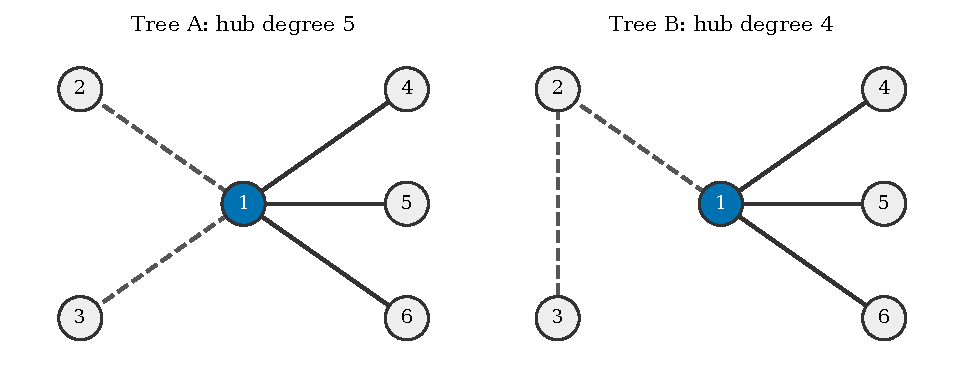
\includegraphics[width=\textwidth]{Fig1.pdf}
\caption{Two of the three optimal trees in Example~\ref{ex:hub}. Solid dark edges occur in all optimal trees; dashed edges are the selected triangle connections. Vertex 1 remains the unique hub although the tree is not identified.}\label{fig:example}
\end{figure}

\section{Calibration of the input band}\label{sec:calibration}
\subsection{Finite-sample inference for independent observations}
The coverage-transfer theorem separates combinatorial computation from statistical calibration. An elementary finite-sample construction is available for Kendall's $\tau_a$. For independent identically distributed vectors $X_1,\ldots,X_n$, define
\[
 \widehat\tau_{ij}={1\over {n\choose2}}\sum_{s<t}
 \operatorname{sign}(X_{si}-X_{ti})\operatorname{sign}(X_{sj}-X_{tj}),
\]
using $\operatorname{sign}(0)=0$. Let $\tau_{ij}$ be the expectation of this kernel.

\begin{corollary}[Finite-sample simultaneous Kendall envelopes]\label{cor:kendall}
For $n\ge2$ set
\begin{equation}\label{eq:kendall}
 \epsilon_{n,m,\alpha}=\sqrt{\frac{2\log(2m/\alpha)}{\lfloor n/2\rfloor}},\quad
 L_e=\max(-1,\widehat\tau_e-\epsilon_{n,m,\alpha}),\quad
 U_e=\min(1,\widehat\tau_e+\epsilon_{n,m,\alpha}).
\end{equation}
The resulting degree and rank envelopes cover all population Kendall-optimal trees simultaneously with probability at least $1-\alpha$, without moment assumptions and allowing tied observations.
\end{corollary}
\begin{proof}
The order-two bounded-kernel inequality of \citet{hoeffding1963} gives
\(\Prob(|\widehat\tau_e-\tau_e|>t)\le2\exp\{-\lfloor n/2\rfloor t^2/2\}\).
It follows by representing the U-statistic as the average over permutations of means of $\lfloor n/2\rfloor$ disjoint-pair kernels, applying the bounded-variable exponential bound and Jensen's inequality. A union bound over the $m$ edges with $t=\epsilon_{n,m,\alpha}$ yields coverage of the entire weight vector. Theorem~\ref{thm:coverage} completes the proof.
\end{proof}
This finite-sample guarantee assumes independence across observations. It is not applied to the serially dependent stock-return windows below. Under the continuous elliptical models used in our independent simulations, $\tau_{ij}=(2/\pi)\arcsin(\rho_{ij})$, so Kendall and Pearson weights have the same population-optimal trees; related invariance is discussed by \citet{kalyagin2022}. Outside such a model, they define different targets.

\subsection{A block-bootstrap implementation for Pearson correlations}
For the practical implementation, let $z_e=\operatorname{atanh}(\rho_e)$ and define $\theta_e=z_e-m^{-1}\sum_f z_f$. Both transformations preserve the set of optimal trees. Subtracting the average transformed correlation removes a common-shift direction that cannot affect a tree. It does not change the population target or eliminate dependence between coordinates.

Compute $\widehat\theta$ and $B$ bootstrap replicates $\widehat\theta^{*(b)}$. All variables, including an observed factor, share the same resampled observation indices. Let $\widehat s_e$ be the standard deviation of the $B$ replicated estimates and define
\begin{equation}\label{eq:maxstat}
 M^{*(b)}=\max_e\left|\frac{\widehat\theta^{*(b)}_e-\widehat\theta_e}{\widehat s_e}\right|,
 \quad q^*=\widehat Q_{1-\alpha}(M^*),\quad
 [L_e,U_e]=[\widehat\theta_e-q^*\widehat s_e,\widehat\theta_e+q^*\widehat s_e].
\end{equation}
The standard errors are fixed across replicates; there is no nested bootstrap studentization. We use the higher empirical quantile. For serially dependent observations, resampling concatenates circular blocks of joint rows and truncates to $n$ observations, following the block-resampling principle of \citet{kunsch1989}.

The statistical qualification is explicit. For fixed $p\ge3$, assume positive variances, correlations strictly inside $(-1,1)$, a joint central limit theorem for the relevant sample moments, consistent estimates of positive asymptotic standard errors for the centered weights, and conditional bootstrap consistency for their joint limit. Also assume continuity of the limiting distribution of the maximum standardized error at its $1-\alpha$ quantile. Under these assumptions, the smooth moment-to-correlation and centering maps imply
\begin{equation}\label{eq:bootstrapassumption}
 \Prob\!\left(\max_e\left|\frac{\widehat\theta_e-\theta_e}{\widehat s_e}\right|\le q^*\right)\longrightarrow1-\alpha
\end{equation}
as $n,B\to\infty$. For a block implementation the block length must also meet the requirements of the relevant bootstrap theorem; it cannot remain fixed in a claimed asymptotic argument. Ties between population edge weights do not violate smoothness of the correlation estimator, provided individual correlations stay away from $\pm1$. Projection then handles the nonsmooth tree map.

We use \eqref{eq:bootstrapassumption} as an input calibration condition, not as a new theorem for arbitrary financial time series. The experiments assess its finite-sample approximation. Heavy tails, nonstationarity, large dimension relative to sample size and data-dependent variable selection can all affect that approximation. No high-dimensional or uniform near-tie validity claim is made for this bootstrap implementation. The finite-sample Kendall result has a separate, fully specified scope.

\subsection{When envelopes become informative}
If the population tree $T_0$ is unique, its exchange margin is
\begin{equation}\label{eq:margin}
 \Delta=\min_{e\notin T_0}\left\{\min_{f\in P_{T_0}(e)}w_{0f}-w_{0e}\right\}>0,
\end{equation}
where $P_{T_0}(e)$ is the tree path connecting the endpoints of $e$. For a graph that is already a tree, identification is automatic. If every weight in $\B$ differs from $w_0$ by less than $\Delta/2$ in sup norm, the cycle inequalities stay strict and $\T(\B)=\{T_0\}$. Hence consistent shrinking bands identify the degree vector for fixed separated populations. The remaining rank interval can still reflect a genuine degree tie.

For the Kendall construction, the joint concentration event implies a maximum deviation of $2\epsilon_{n,m,\alpha}$ throughout the box. Thus $4\epsilon_{n,m,\alpha}<\Delta$ is a sufficient condition for tree identification on that event. It is not necessary for hub identification, as Example~\ref{ex:hub} shows. At exact population edge ties, a nontrivial identified set can persist even with unlimited data.

\section{Simulation study}\label{sec:simulation}
\subsection{Design and evaluation targets}
The main experiment uses $p=12$, $n\in\{126,252,1008\}$, $R=500$ independent Monte Carlo replications per design and $B=999$ bootstrap replications per data set, with nominal level 95\%. All 7500 replication-level results and their seeds are retained; the simulated data can be regenerated from those seeds. Simulations are method-development experiments, not a preregistered confirmatory analysis.

For the Gaussian models, $X_{ti}=a_i F_t+\sqrt{1-a_i^2}\varepsilon_{ti}$ with independent standard-normal innovations. The independent model uses $a_i=0$. The separated-star model sets $a_1=0.99$ and spaces the remaining loadings from 0.45 to 0.55. The near-tie design sets $a_1=0.8+0.5/\sqrt n$, $a_2=0.8$ and spaces the others from 0.45 to 0.55. For every finite $n$ the population tree in the latter two designs is the star at vertex 1, by the singleton-cut property. The shrinking loading difference in the near-tie design tests behavior close to loss of identification.

The serial-dependence design applies $X_t=0.4X_{t-1}+\sqrt{1-0.4^2}Z_t$ to Gaussian separated-star innovations, preserving their contemporaneous correlation matrix. The heavy-tail design divides each Gaussian vector by an independent $\sqrt{\chi^2_5/5}$, giving elliptical multivariate $t_5$ observations with the same correlations. Independent models use ordinary row resampling. The autoregressive model uses circular blocks of rounded length $n^{1/3}$, namely 5, 6 and 10.

We report coverage of the entire transformed-weight vector, simultaneous coverage of all population degree endpoints, simultaneous coverage of every permissible rank, average degree width and the size of the candidate set for rank one. Under independence, every labelled tree is population optimal, so the degree target for every vertex is $[1,p-1]$ and the rank target is $[1,p]$. Under the other designs, the population star is unique. This distinction prevents an arbitrary deterministic tree at independence from becoming an artificial ground truth.

Two deliberately simple comparators expose different inferential choices. The first projects marginal 95\% Fisher-scale intervals computed with the same bootstrap standard errors, without simultaneous calibration. The second takes the marginal 2.5\% and 97.5\% empirical quantiles of resampled degrees. The latter is evaluated for simultaneous degree coverage only in unique-tree designs, because its interpretation at a set-identified population target is not specified. Neither comparator is claimed to be the best available ranking procedure. In particular, applying methods for directly estimated smooth population scores to discontinuous tree degrees would require a separate argument.

\subsection{Results and computational verification}
Table~\ref{tab:sim} reports all primary designs. The underlying band coverage ranges from @@BAND_MIN@@\% to @@BAND_MAX@@\%; projected degree coverage ranges from @@DEG_MIN@@\% to @@DEG_MAX@@\%. These are different diagnostics. Conservative graph projection can cover the target even on some draws for which the true weight vector lies outside the input band. It cannot retrospectively turn an undercalibrated band into a generally valid inferential procedure.

@@SIM_TABLE@@

At $n=1008$, the Gaussian separated-star design certifies the true leading vertex in @@STAR_CERT@@\% of replications. At $n=252$, the same rate is @@STAR_SMALL_CERT@@\%, showing the finite-sample cost of the rectangle. In the near-tie model with $n=252$, simultaneous degree coverage of the marginal percentile comparator is @@NEAR_PERCENTILE@@\%, while the proposed degree envelopes cover in @@NEAR_DEG@@\%. This comparison concerns the known population star degree vector, not a causal notion of hub importance. The proposed candidate set remains broad near the tie; that conservatism is visible in Figure~\ref{fig:sim}, rather than being summarized as successful identification.

\begin{figure}[t]
\centering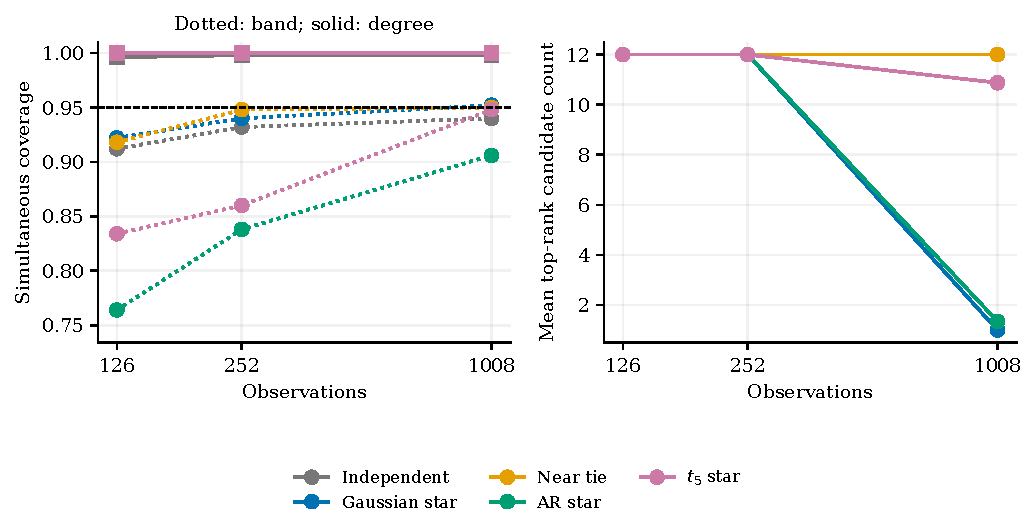
\includegraphics[width=\textwidth]{Fig2.pdf}
\caption{Monte Carlo performance of the centered Fisher-scale projection. Left: coverage of the simultaneous input band and of the entire population degree target. Right: mean number of candidates for the highest degree. Each point uses 500 independent replications; the horizontal reference in the left panel is 0.95.}\label{fig:sim}
\end{figure}

The finite-sample Kendall variant is evaluated separately in 3000 independent data sets, with 500 replications in each of six designs. The designs include independent and near-tie observations at $n=252$, and Gaussian and $t_5$ separated stars at $n=1008$ and 4096. The result is reported in Table~\ref{tab:kendall}. Its guaranteed coverage has a visible price in interval width; no serial-dependence guarantee is inferred from this experiment.

@@KENDALL_TABLE@@

To assess shapes beyond a star, a further 3000 data sets use two Gaussian tree models with the same three sample sizes, 500 replications per cell and 999 resamples. Each variable is generated from its parent by $X_i=b_iX_{\mathrm{parent}(i)}+\sqrt{1-b_i^2}\varepsilon_i$. In the chain, $b_i=0.75$. In the two-hub tree, vertices 1 and 2 are joined with coefficient 0.5; five additional leaves attach to each hub with coefficient 0.7. Correlations equal products along paths, so the population maximum-correlation tree is the generating tree. The two largest degrees are tied in the two-hub model, and ten degrees are tied for first place in the chain. Evaluation retains these rank ties. Table~\ref{tab:shapes} reports the additional designs; their purpose is to measure performance on distinct topologies, not to select a favorable application.

@@SHAPE_TABLE@@

For every coverage estimate $\widehat c$, the reported replication files allow binomial uncertainty to be reconstructed; Wilson intervals are included in the summary data. At $R=500$, a coverage probability of 0.95 has Monte Carlo standard error approximately 0.0097. Zero observed failures therefore do not establish coverage equal to one.

An independent exhaustive verification enumerates all labelled trees on 3--6 vertices and tests 1040 randomly generated integer interval boxes, including zero-width intervals and exact ties. For each candidate tree, optimality is checked at its own favourable endpoint configuration, rather than through the vertex-envelope algorithm. All degree extrema agree, covering 11244 feasible tree witnesses. Weighted bootstrap covariance calculations are also checked against direct resampling and refitting of the factor regression; the largest absolute covariance discrepancy is below $10^{-14}$. These checks support the implementation and complement the proofs; they do not prove novelty or replace the statistical assumptions.

\section{Application to Polish equity correlations}\label{sec:gpw}
\subsection{Observed data and representations}
We reanalyse the previously assembled histories underlying a study of hub stability and diversification risk. Historical WIG20 and mWIG40 quarterly portfolio snapshots identify the candidate universe. Available company and WIG price histories were obtained from Bankier's public quotation service, with source metadata and hashes retained in the accompanying repository. Observations end in 2025. Among 171 recorded security identities, histories were available for 164; 155 securities enter at least one of the 231 retained estimation windows during 2007--2025. The networks contain 41--60 securities, with mean 51.9, and use 252 sessions of complete past returns.

The original eligibility rules require complete past returns and volumes, positive volume on at least 90\% of sessions, no more than 15\% zero close-to-close returns, and positive return variance. They were applied to both close-to-close and open-to-close conventions in the original analysis; this extension retains the resulting universe and uses close-to-close log returns. No unavailable quotation is imputed. The new calculations do not require future portfolio outcomes, so all 231 network windows are retained.

Three representations are examined: raw returns, returns minus the contemporaneous cross-sectional average, and residuals from an intercept-and-WIG regression fitted within each window. For the last representation, joint resampling of the stocks and WIG refits the regression in every replicate. Equivalently, its covariance is computed from the resampled joint covariance as $\widehat\Sigma_{XX}-\widehat\Sigma_{XF}\widehat\Sigma_{FF}^{-1}\widehat\Sigma_{FX}$. For cross-sectional subtraction, $M\widehat\Sigma M$ is used, with $M=I-\mathbf1\mathbf1'/p$. These representations define different population targets.

The identity $(M\Sigma M)\mathbf1=0$ explains why cross-sectional subtraction constrains correlations. A one-factor model can likewise generate a stable star without residual cross-asset dependence. These are established algebraic diagnostics, not the methodological novelty claimed here. Their role is to clarify which network is being ranked, including the transformation used in \citet{galazka2011}.

Primary bands use $B=999$ circular joint block replicates of length 10 and nominal level 95\%. Calibration is performed separately for each window and representation, jointly over its edge weights. There is no familywise claim across the 231 dates or across the three representations. The theoretical bootstrap justification concerns a fixed variable set and an appropriate stationary sampling model. The empirical eligibility filter is data dependent, and local stationarity is an approximation; coverage conditional on passing that filter is not established. Accordingly, all reported application intervals are nominal bootstrap intervals.

\subsection{What the data resolve under this procedure}
Table~\ref{tab:gpw} shows the main result. Every rank interval is $[1,p]$, so $C_k=V$ and $D_k=\varnothing$ for $k=\lceil0.1p\rceil$ in every window and representation. Mean degree-envelope widths are approximately 47.3 for raw returns, 47.5 after cross-sectional subtraction and 48.4 after WIG residualization. These are wide relative to the attainable degree range $[1,p-1]$.

@@GPW_TABLE@@

For context, the earlier calculation with 500 block replicates and fractional handling of ties selected at least one top-decile hub with frequency at least 0.80 in 129 raw-return windows, five demeaned windows and eight residual windows. Those saved frequencies are retained as descriptive comparators and are not recalculated with $B=999$. The present confidence construction certifies none of those vertices as belonging to every admissible top-decile set. This does not show that the selection frequencies were computed incorrectly: selection stability and confidence coverage answer different questions.

\begin{figure}[t]
\centering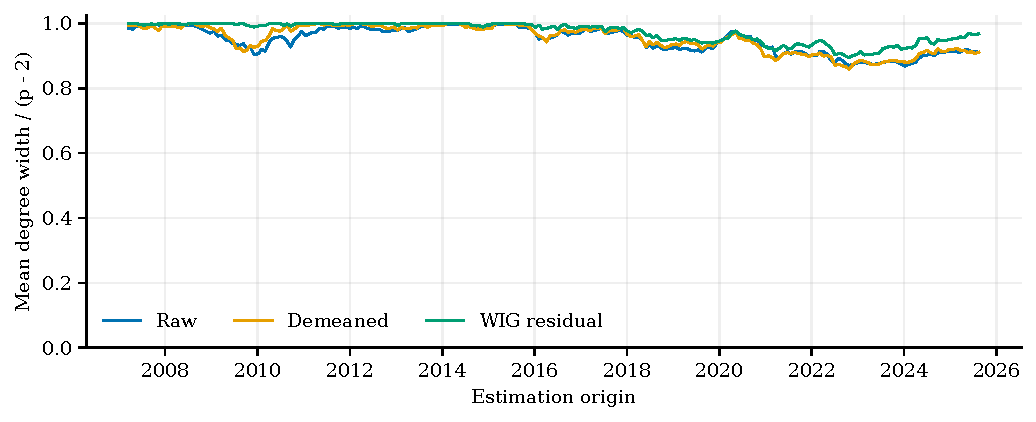
\includegraphics[width=\textwidth]{Fig3.pdf}
\caption{Mean degree-envelope width divided by the maximum possible width $p-2$ in each GPW window. The uncertainty sets remain broad in all three representations. Overlapping windows produce dependent points; the figure is descriptive and carries no simultaneous inference over time.}\label{fig:gpw}
\end{figure}

Block-length sensitivity uses lengths 5 and 20 on every fifth retained origin, a fixed subsample of 47 windows spread across the observation period. @@GPW_SENSITIVITY@@ This check addresses a tuning choice within the same conservative rectangular method; it does not establish adequate calibration under all forms of nonstationarity.

The earlier exploratory forecasting exercise used 73 complete test outcomes during 2019--2025. Adding residual-network selection reliability changed mean squared error by +2.20\%, while an open-to-close sensitivity estimate changed it by -2.69\%; both paired intervals included zero. These inherited findings and their original code remain available in the repository. They motivate caution about financial interpretation but are not a new forecast result or evidence supporting the confidence method.

\subsection{Data limitations}
Membership follows archived quarterly portfolios rather than a fully reconciled daily history of all extraordinary replacements. Prices are used as supplied and are not certified cash-dividend-inclusive total returns. The original data audit compared 4241 downloaded closing prices against GPW portfolio documents: 3950 matched strictly, 33 additionally matched at the documents' whole-zloty precision, 253 differences were consistent with denomination changes and five remained unresolved. This check supports identity and scale matching, not a complete corporate-action audit. Across the full downloaded source histories, 590 of 751158 security-day records failed open-high-low-close or volume checks and were treated as missing. The study cutoff and eligibility restrictions were then applied.

Downloaded historical prices may incorporate later adjustments. The seven unavailable histories and complete-case filtering can affect representativeness, and the single WIG factor is only one possible adjustment. In particular, nominal coverage cannot be inferred from a public data source, from the absence of imputation, or from the implementation checks. The empirical conclusion is limited to how informative this particular uncertainty construction is on the retained historical windows.

\section{Discussion}\label{sec:discussion}
The central computational result is that a seemingly large projection over all interval-compatible optimal trees has exact degree endpoints obtainable from only two extremal configurations per vertex. Coupled with a valid simultaneous band, this gives confidence envelopes without assigning a spurious unique tree to a tied population. It also permits a distinction between certifying a hub and recovering every edge of its tree.

The main limitation is geometric. Coordinatewise bands sacrifice the dependence structure of joint estimation when their rectangular region is projected. The shared bootstrap quantile accounts for multiplicity in constructing the band, but it does not retain an ellipsoidal or other joint shape. In addition, the projection admits weight vectors outside the correlation-matrix constraint. Finally, combining separate degree endpoints into rank bounds introduces a further relaxation. Each step can enlarge the final set without lowering coverage on the joint-band event. The GPW result shows that this cost can dominate the application.

Input calibration is a separate limitation. The bootstrap coverage estimates in Table~\ref{tab:sim} are not uniformly equal to their nominal value. Finite-sample undercoverage, especially under dependence or heavy tails, remains a concern even when projected degree coverage is high. The Kendall construction gives a genuine finite-sample guarantee under independent sampling, but its uniform concentration radius can be substantially more conservative. We therefore report the bootstrap as an asymptotic implementation with measured finite-sample performance, and the Kendall version as an independent-observation guarantee.

Several extensions are natural research problems. Projection onto a correlation-constrained joint confidence region could improve precision, but its exact computational cost must be addressed. Confidence regions for selected edge-order contrasts may exploit cancellations unavailable to coordinatewise bands. Sharper rank bounds could retain the joint feasibility of competing degree extrema. Any such extension needs a coverage argument for the intended target and should be assessed by both error control and set size. Simply lowering a selection-frequency threshold would not provide that argument.

For applied reporting, a stable displayed hub and a narrow confidence set should be reported as distinct findings. Broad sets can be scientifically informative when they reveal that available observations do not support a precise ranking under a stated method. They should not be represented as evidence of equal economic influence, causal transmission or predictive value. The present results establish a tractable projection and document where it succeeds and where its uncertainty region is too broad to resolve the applied question.

\section*{Statements and Declarations}
\subsection*{Funding}
No dedicated funding was received for this work.
\subsection*{Competing interests}
The authors have no competing interests relevant to this work.
\subsection*{Data and code availability}
Code, seeds, replication-level outputs, derived GPW intervals and verification records are available at \url{https://github.com/mgalazka84/gpw-hub-reliability/tree/statpapers-v0.2.1}, in the \texttt{statistical\_papers} directory. The earlier empirical acquisition and audit are preserved at tag \texttt{v1.0.1}. Third-party price panels and GPW portfolio documents are not redistributed; their source links, acquisition instructions and hashes are provided. Later provider revisions may prevent byte-identical reacquisition. The data providers are Bankier.pl (\url{https://www.bankier.pl/inwestowanie/profile/quote.html?symbol=PKOBP}) and GPW Benchmark (\url{https://gpwbenchmark.pl/historyczne-portfele-indeksow}).
\subsection*{AI assistance}
ChatGPT (OpenAI) assisted with coding, data handling, methodological development and manuscript drafting. The authors are responsible for the submitted work.

% Include the bibliography style's settings entry without a printed citation.
% Every research reference in this file is also cited in the text.
\nocite{*}
\bibliography{references}
\end{document}
